\begin{document}
\begin{figure}[H]
  % \makebox[\textwidth][c]{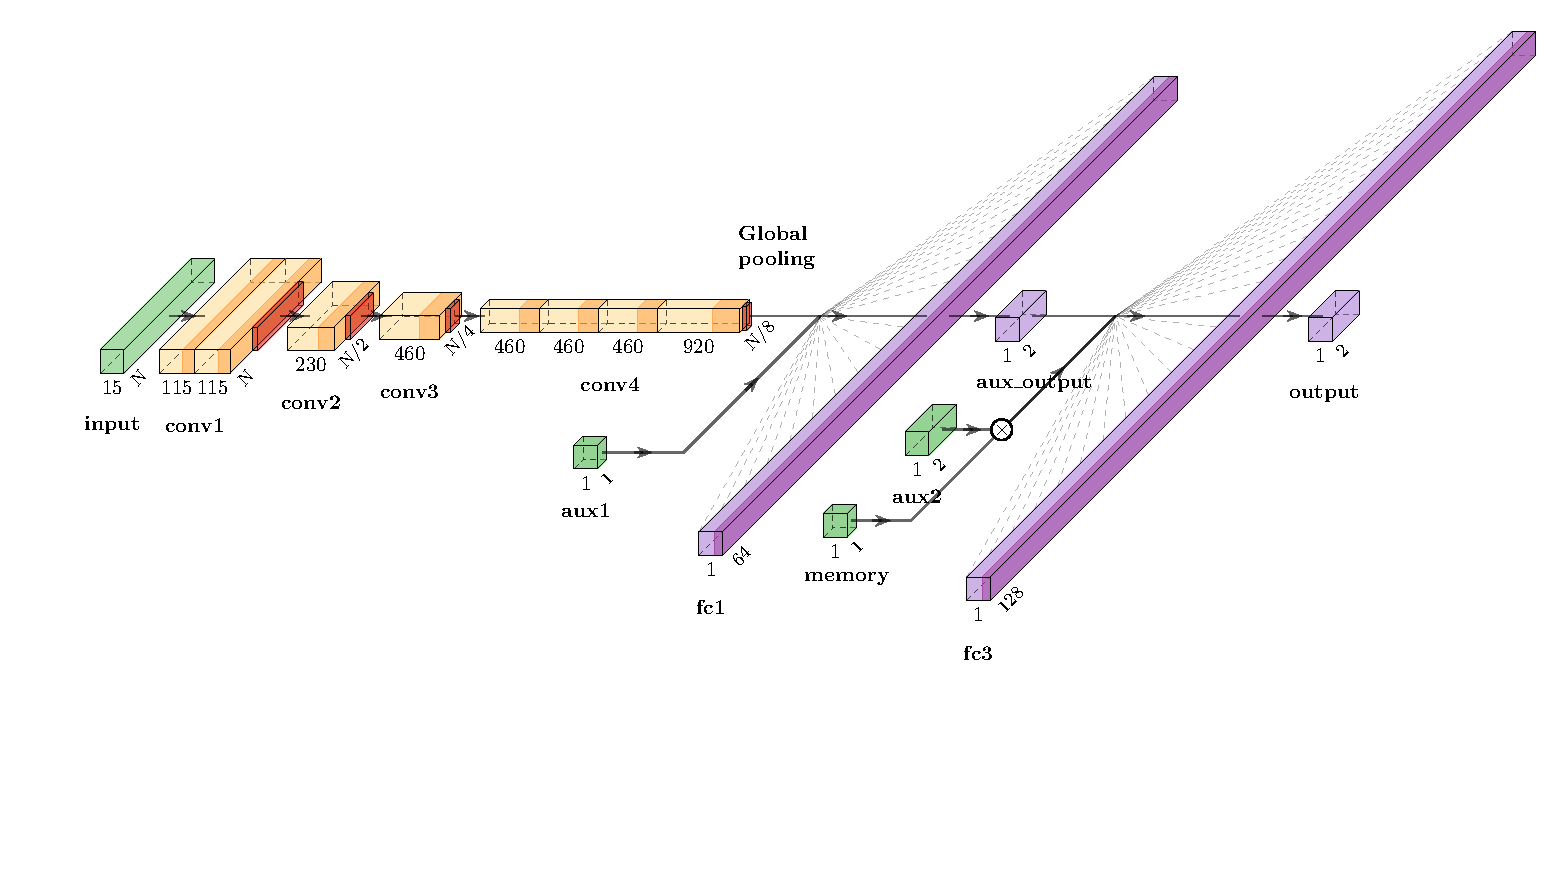
\includegraphics[width=1.0\textwidth]{./img/architettura.pdf}}%
  \makebox[\textwidth][c]{%
    \includetikz{0.75}{./img/architettura}%
  }%
  % 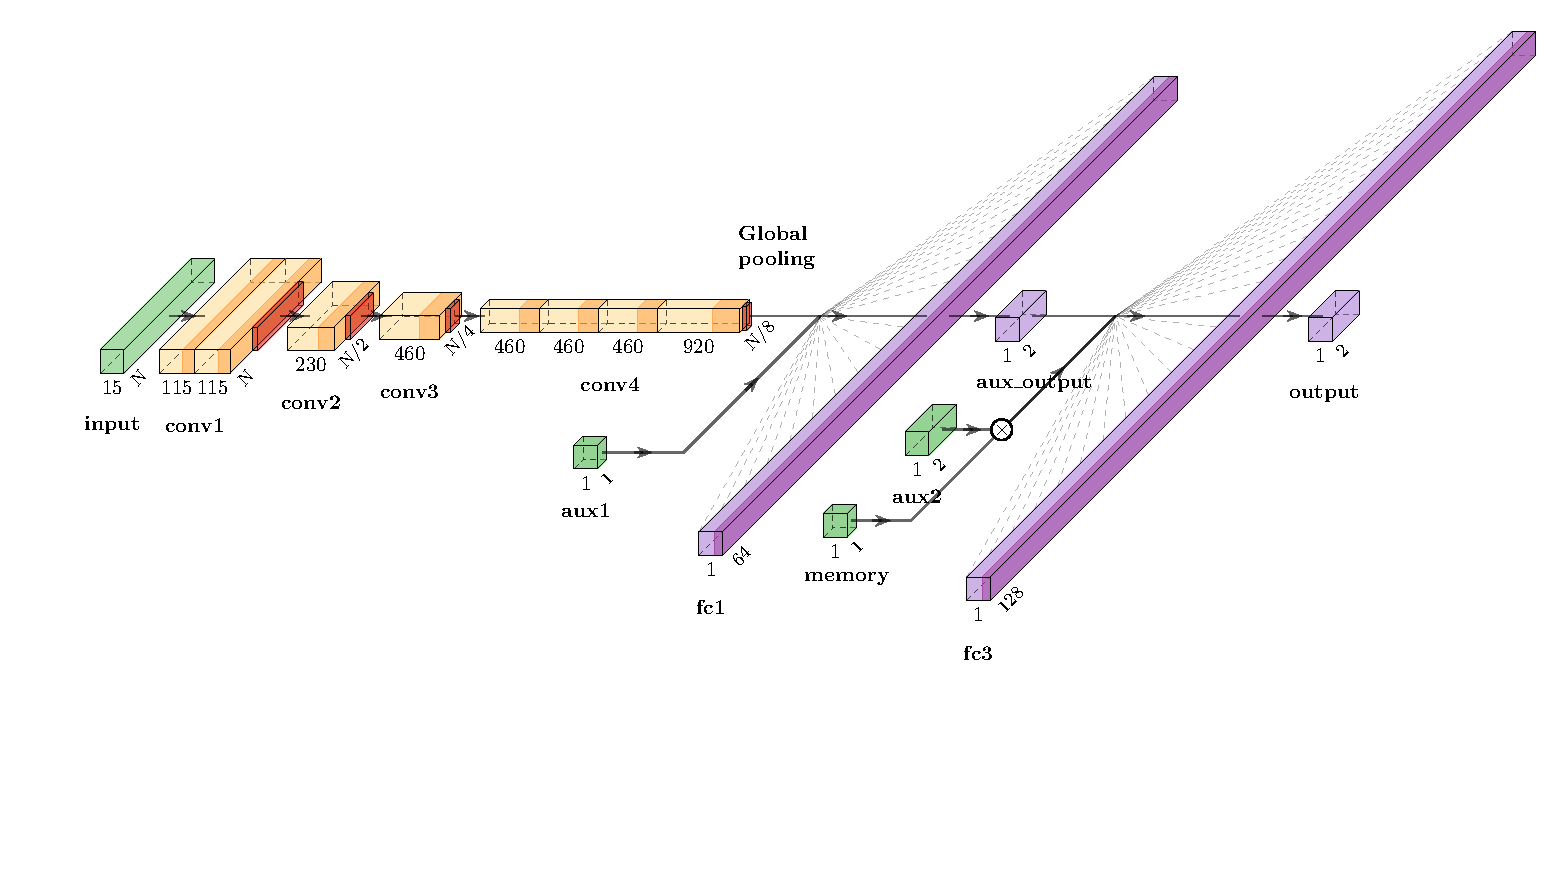
\includegraphics[width=1.3\textwidth]{./img/architettura.pdf}
  % \includetikz{0.8}{./img/architettura.tex}
  \caption{Architettura della rete neurale}%
  \label{fig:crynet}%
\end{figure}
In questo capitolo è descritta nel dettaglio l'architettura software sviluppata
per il progetto di locallizazione indoor, inclusa la rete neurale, le librerie
utilizzate, gli ambienti di sviluppo e gli strumenti che hanno coadiuvato il
testing e la sperimentazione del prototipo.
\section{TensorFlow}
%%%%%%%%%%%%%%%%%%%%%%%%%%%%%%%%%%%%%%%%%%%%%%%%%%%%%%%%%%%%%%%%%%%%%%%%%%%%%%%
\section{Keras}
%%%%%%%%%%%%%%%%%%%%%%%%%%%%%%%%%%%%%%%%%%%%%%%%%%%%%%%%%%%%%%%%%%%%%%%%%%%%%%%
\section{Google Colab}
%%%%%%%%%%%%%%%%%%%%%%%%%%%%%%%%%%%%%%%%%%%%%%%%%%%%%%%%%%%%%%%%%%%%%%%%%%%%%%%
\section{Weights \& Biases}
%%%%%%%%%%%%%%%%%%%%%%%%%%%%%%%%%%%%%%%%%%%%%%%%%%%%%%%%%%%%%%%%%%%%%%%%%%%%%%%
\section{Rete Neurale Utilizzata}
La rete neurale sviluppata per il problema di localizzazione indoor è
illustrata schematicamente in Figura~\ref{fig:crynet}. Essa consiste in una
serie di blocchi convoluzionali seguiti da alcuni livelli di neuroni
completamente connessi. Il modello sfrutta, oltre ai segnali RSSI emessi dai
beacon, anche due input ausiliari che non sono processati dalla sezione
convoluzionale della rete.
\subsection{Input del Modello}
L'input principale del modello è composto da una serie temporale di valori RSSI
di 15 beacon disposti lungo il perimetro dell'edificio dell'ASL, nel quale si
sono svolte le sperimentazioni del prototipo. La dimensione temporale
dell'input può essere arbitrariamente lunga, poichè una sua variazione
determina solamente una differente dimensione dell'asse temporale dell'output
della CNN\@. La sezione convoluzionale della rete si conclude infatti con un
livello di pooling globale che consiste nell'estrarre, per ogni feature map
prodotta, la media aritmetica dei valori di input lungo la dimensione del
tempo. Come si vede in Figura~\ref{fig:crynet}, infatti, la dimensione
dell'output di tale livello è sempre costante e risulta essere $920\times1$.

A completare l'input del modello sono il valore emesso, nel momento
dell'utilizzo del modello, dal sensore magnetico dello smartphone e
l'ultima posizione nota dell'utente all'interno dell'edificio. Il valore della
bussola è utile per determinare l'orientamento della persona nello spazio,
rendendo la rete neurale capace di considerare le variazioni dei segnali BLE
dovuti all'assorbimento da parte del corpo dell'utilizzatore dello smartphone.
Il secondo input ausiliario è invece utilizzato per correggere eventuali grandi
scostamenti dell'output della CNN rispetto alla posizione precedente
dell'utente. Ci si aspetterebbe infatti che tale posizione non variasse di
molto in un lasso di tempo sufficientemente breve.

L'ultima posizione nota dell'utente viene pesata da un coefficiente, anche esso
input del modello, che in Figura~\ref{fig:crynet} è indicato con la lettera
greca \(\mu\). Tale valore, a cui possiamo riferirci con il termine
\emph{coefficiente di memoria residua}, è compreso tra zero e uno, e determina
il peso che si vuole dare all'ipotesi di continuità della posizione dell'utente
nel tempo.  \(\mu = 0\) indica l'assenza di tale assunzione, con la conseguente
massima riduzione della correzione dell'output della CNN da parte dei livelli
successivi, mentre \(\mu = 1 \) associa il massimo peso su tale ipotesi. Il
coefficiente di memoria residua è esso stesso input del livello successivo
della rete, il quale riceve anche i valori dell'output ausiliario e di \( \mu
  \cdot \bm y'\), dove con \(\bm y'\) si indica la posizione precedente dell'utente.
\subsection{Blocco Convoluzionale}
\subsection{Uso della Bussola e Output Ausiliario}
\subsection{Coefficiente di Memoria Residua e Input Ausiliario}
\subsection{Output del Modello}
%%%%%%%%%%%%%%%%%%%%%%%%%%%%%%%%%%%%%%%%%%%%%%%%%%%%%%%%%%%%%%%%%%%%%%%%%%%%%%%
\section{Dataset Augmentation e Preprocessing}
\subsection{Jittering}
\subsection{Ridimensionamento (Scaling)}
\subsection{Magnitude Warping}
\subsection{Permutazione di Sottoinsiemi (Subset Shuffling)}
\subsection{Deattivazione Selettiva}
%%%%%%%%%%%%%%%%%%%%%%%%%%%%%%%%%%%%%%%%%%%%%%%%%%%%%%%%%%%%%%%%%%%%%%%%%%%%%%%
\section{Addestramento del Modello}
%%%%%%%%%%%%%%%%%%%%%%%%%%%%%%%%%%%%%%%%%%%%%%%%%%%%%%%%%%%%%%%%%%%%%%%%%%%%%%%
\section{Ensembling}
%%%%%%%%%%%%%%%%%%%%%%%%%%%%%%%%%%%%%%%%%%%%%%%%%%%%%%%%%%%%%%%%%%%%%%%%%%%%%%%
\section{Compilazione e Deploy del Modello}

\end{document}
